\label{chap:pdp_protocol}

This chapter discusses the underlying communication details of the packetized display protocol (PDP) architecture. First, it gives an overview of the protocol design methodology. Secondly, it provides comparison with conventional display technology. Thirdly, it discusses requirements for packet formatting. Fourthly, it discusses individual packet types. Fifthly, it delves into the overhead of utilizing PDP packets. Sixthly, it discusses multi-frame rate performance within the PDP through an example of a dual frame rate operation. The central purpose of this chapter is to provide the reader with an understanding of the reasoning behind design decisions as well as to provide a detailed specification of the protocol and its performance characteristics when utilized in different scenarios.

\section{Design Methodology}
    \label{sec:design_methodology}
    This section discusses the design methodology for the PDP Protocol which began with a number of critical design goals~\cite{LandwehrEtAl2019}. An attempt to address the goals is not presented directly here but discussed  elsewhere due to it being a complex topic with many interwoven aspects. The design goals are as follows:

    \begin{enumerate}
        \item {\em To design a scalable display system that is distributable and hardware agnostic.} The display protocols and interfaces utilized within projector systems have systematic issues with remaining up to date with current technology in that old standards (such as DVI) continue to be utilized due to the inability for custom synchronization solutions to work with newer hardware as well as due to the costs and time associated with implementing newer solutions utilizing newer standards. This is touched upon throughout this chapter and discussed more extensively in Chapter~\ref{chap:machine_model}.
        \item {\em To provide a protocol that is relatively simple to implement without unnecessary complexity to ease the encoding and decoding process.} A low overhead and fast decode process is crucial to ensuring latency is sub-frame\footnote{This refers to latency of that below the time it would take to buffer an entire frame.} across an end-to-end system. Additionally, simplifying these processes also eases potential hardware implementation mistakes as well as inefficiencies that could lead to reduced performance. This is discussed in Chapters~ \ref{sec:packet_format},~\ref{sec:packet_types}, and~\ref{sec:pdp_stream_decoding}.
        \item {\em To provide dynamic intra-frame variable refresh rate (VRR) in order to enable better bandwidth utilization.} In particular, to allow for regions of a display to be intelligently updated at different rates when driven by a scene generator. This is discussed upon in Chapters~\ref{sec:multi_framerate_performance} and \ref{sec:compositing}.
        \item {\em To provide a path to utilize conventional display protocol streams such as HDMI as a backwards compatible transport layer for the PDP without introducing overhead.} This is to allow for interoperability where necessary when utilizing conventional display sources, and to ease migration to a PDP based system. This is touched upon in Chapter~\ref{sec:pdp_stream_decoding} and discussed more extensively in Chapter~\ref{chap:implementation}.
    \end{enumerate}

    For methodology, each goal was considered when making decisions about what should and should not be part of the PDP, and where the boundaries of the protocol should lie. This included such decisions as how to incorporate hardware specific features, the best method to support VRR without constraining the methods by which users can implement support for it within scene generators\footnote{VRR implemented within HDMI and DisplayPort is driver controlled and thus the user has no ability to control it.}, and how to ease implementation in current and future hardware. Hardware specific optimizations can be important for performance reasons even in hardware agnostic protocols. Therefore, it is paramount to make hardware agnostic protocols general enough to support various configurations. For example, tuning within TCP~\cite{WeigleFeng2002} is a well-known important consideration in the field of networks for maximizing throughput due to differing hardware and network topologies. In the PDP, one example of a hardware specific feature that needs consideration is the support for different array write processes\footnote{See Chapter~\ref{chap:array_write_process} for the interleaved array write process of the NSLEDS and HDILED arrays.} because efficient ordering of data is important for low-latency operation and minimizing hardware complexity.

\section{Comparison}

    To better understand how to design the PDP, the constraints of conventional display protocols were investigated to discern which features within these protocols conflict with the design goals of the PDP. In addition, it was necessary to investigate whether these could provide a path forward in the design and development of the PDP. Many versions of these protocols (DVI~\cite{DDWG1999}, HDMI~\cite{HDMIForum2018}, DisplayPort~\cite{VESA2016}, etc.) provide similar feature-sets to end-users with the major focus being on increasing refresh rates and resolutions with each new specification. However, as discussed in Chapter~\ref{sec:conventional_display_protocols}, their basis is rooted in classical analog video specifications that utilize scan lines~\cite{Neal1998}. This means that signal timing utilizes vertical and horizontal blanking periods that consist of a front-porches, sync pulses, and back-porches; in addition to, the active video data to be displayed.

    For early analog display devices, these signals enabled operators to manually adjust horizontal and vertical hold times relative to the sync pulses to correct for the imprecise timing of early display hardware; but provide little benefit on modern hardware other than as an embedded method to support sending frames at a static interval, and to enable tearless buffer swapping in either double buffering~\cite{FriedbergEtAl1990} or triple buffering schemes~\cite{3dfx1997} utilized within GPUs\footnote{This is performed by swapping buffers during the vertical sync (vsync) interval of a frame~\cite{3dfx1999,3dfx1999_2}. See Chapter~\ref{chap:display_protocols} for details about vsync intervals.}.

    In digital display technology, embedded blanking periods represent an anachronism that impedes the goal of maximizing bandwidth utilization when driving a display by requiring the transmission of unnecessary data over digital protocols. For example, a commonly utilized 1920 by 1080-pixel mode operating at \mbox{60 hertz}~\cite{MythTV2015} on a modern display has a 16 percent blanking period overhead due to the specification of vertical and horizontal sync periods. Other examples can be seen in Table~\ref{tbl:modeline_overhead}. Of note, modes with {\it 512 by 512} and {\it 512 by 256} visible pixels are non-standard and were tested on existing hardware to minimize the overhead of blanking. Additionally, these have been utilized within NSLEDS and TCSA during actual array operation. What one sees is that as modelines shrink and data rates decrease, the percentage of blanking relative to displayed pixels significantly increases. This is due to the inability for common implementations of video decoders to operate correctly when blanking is minimized. An additional issue is that when non-standard visible resolutions are utilized many decoders do not operate at all.

    \begin{table}
        \centering
        \large
        \begin{tcolorbox}[tabularx={Y|Y|Y|Y|Y},title=\textbf{Modeline Overhead},boxrule=0.5pt]
        \textbf{\normalsize Resolution} & \textbf{\normalsize Refresh Rate (Hz)} & \textbf{\normalsize Visible Pixels} & \textbf{\normalsize Total Pixels} & \textbf{\normalsize Overhead} \\ \hline
            \textbf{\normalsize 1920x1080} & \textbf{\normalsize 60}   & {\normalsize 2073600} & {\normalsize 2475000} & {\normalsize 16.2\%} \\ \hline
            \textbf{\normalsize 1600x1200} & \textbf{\normalsize 60}   & {\normalsize 1920000} & {\normalsize 2700000} & {\normalsize 28.9\%} \\ \hline
            \textbf{\normalsize 1280x1024} & \textbf{\normalsize 60}   & {\normalsize 1310720} & {\normalsize 1799408} & {\normalsize 27.2\%} \\ \hline
            \textbf{\normalsize 1280x960}  & \textbf{\normalsize 60}   & {\normalsize 1228800} & {\normalsize 1800000} & {\normalsize 31.7\%} \\ \hline
            \textbf{\normalsize 1280x800}  & \textbf{\normalsize 60}   & {\normalsize 1024000} & {\normalsize 1391040} & {\normalsize 26.4\%} \\ \hline
            \textbf{\normalsize 1024x768}  & \textbf{\normalsize 60}   & {\normalsize 786432 } & {\normalsize 1083264} & {\normalsize 27.4\%} \\ \hline
            \textbf{\normalsize 512x512}   & \textbf{\normalsize 500}  & {\normalsize 262144 } & {\normalsize 296100 } & {\normalsize 11.5\%} \\ \hline
            \textbf{\normalsize 512x512}   & \textbf{\normalsize 400}  & {\normalsize 262144 } & {\normalsize 296100 } & {\normalsize 11.5\%} \\ \hline
            \textbf{\normalsize 512x512}   & \textbf{\normalsize 300}  & {\normalsize 262144 } & {\normalsize 357500 } & {\normalsize 26.7\%} \\ \hline
            \textbf{\normalsize 512x512}   & \textbf{\normalsize 100}  & {\normalsize 262144 } & {\normalsize 357500 } & {\normalsize 26.7\%} \\ \hline
            \textbf{\normalsize 512x512}   & \textbf{\normalsize 60}   & {\normalsize 262144 } & {\normalsize 357500 } & {\normalsize 26.7\%} \\ \hline
            \textbf{\normalsize 512x512}   & \textbf{\normalsize 50}   & {\normalsize 262144 } & {\normalsize 364000 } & {\normalsize 28.0\%} \\ \hline
            \textbf{\normalsize 512x512}   & \textbf{\normalsize 30}   & {\normalsize 262144 } & {\normalsize 520000 } & {\normalsize 50.0\%} \\ \hline
            \textbf{\normalsize 512x256}   & \textbf{\normalsize 1000} & {\normalsize 131072 } & {\normalsize 149460 } & {\normalsize 12.3\%} \\ \hline
            \textbf{\normalsize 512x256}   & \textbf{\normalsize 500}  & {\normalsize 131072 } & {\normalsize 256000 } & {\normalsize 48.8\%} \\ \hline
            \textbf{\normalsize 512x256}   & \textbf{\normalsize 200}  & {\normalsize 131072 } & {\normalsize 320000 } & {\normalsize 59.0\%} \\ \hline
            \textbf{\normalsize 512x256}   & \textbf{\normalsize 100}  & {\normalsize 131072 } & {\normalsize 320000 } & {\normalsize 59.0\%} \\ \hline
            \textbf{\normalsize 512x256}   & \textbf{\normalsize 60}   & {\normalsize 131072 } & {\normalsize 320000 } & {\normalsize 59.0\%} \\ \hline
        \end{tcolorbox}
        \caption[Modeline Overhead]{Modeline overhead for various resolutions and refresh rates~\cite{MythTV2015}. Computed using active pixel area over total pixel area. 512x512 and 512x256 are typical modeline resolutions used on IRLED arrays.}
        \label{tbl:modeline_overhead}
    \end{table}

    These protocols also internally utilize a mode based display of data that requires the specification of the absolute width and height of display as well as a pixel clock which when used in conjunction with the vertical blanking information provides a total refresh rate as described in Chapter~\ref{sec:conventional_display_protocols}. This means that the bandwidth requirements for a given mode are inherently static across all frames. In addition, this constrains the refresh rate for a display to be static in terms of both the intra-frame regions of the display and between frames. Effectively increasing the burden of synchronization and impeding the introduction of dynamism into the display process.

    In recent years, work has been done to implement a limited form of variable refresh rate (VRR) display between frames for use with newer protocols~\cite{AMD2019,NVIDIA2020_1}. In essence, it allows for entire frames to be sent for display immediately once the rendering process has completed. A downside is that historically this has generally required specialized hardware support out of the scope of protocol specifications. A recent update of the HDMI 2.1 specification~\cite{HDMIForum2018} has integrated a speed-limited form of VRR directly into the specification that requires full frames of data to be transmitted at a statically specified resolution and target frame rate. DisplayPort provides a similar form of VRR~\cite{VESA2014} with a similar set of limitations which also require full frames of data to be transmitted at a specified resolution and target frame rate.

    DisplayPort differs from older display standards in that data streams themselves are framed~\cite{VESA2011,Wiley2011}, though the standard itself refers to this framing as packetization it differs from the normal sense of packets in that arbitrary packets of data with dynamic meanings and decoding cannot be sent. An example of the framing is shown in Figure~\ref{fig:display_port_framing}. Once per frame in between pixel data, a {\it blanking start} symbol is inserted into the data stream to indicate the start of vertical blanking. Then, a {\it Main Stream Attribute (MSA)} packet is sent that contains the total number of horizontal pixels per line, the total number lines, the start of active video pixels relative to hsync, the start of active lines relative to vsync, and the pixel formatting. After which, a {\it blanking end} symbol is inserted to indicate the end of vertical blanking. Following this, pixel data conforming to the video specification within the MSA packet is sent along with {\it stuffing} symbols that are framed with {\it fill start} and {\it end} symbols. These can be of different lengths and are used to represent space between actual data. After all the data for a frame is sent, {\it blanking} symbols for the next frame occur, and the process repeats. In essence, what DisplayPort provides is a framed method of sending video formatting information per frame instead of embedding these signals in a separate synchronized stream. Display port also provides a secondary stream to send audio or other information (not shown) during the blanking interval similar to how blanking intervals are sometimes used as a side channel for extra data in earlier protocols.

    \begin{figure}
        \centering
        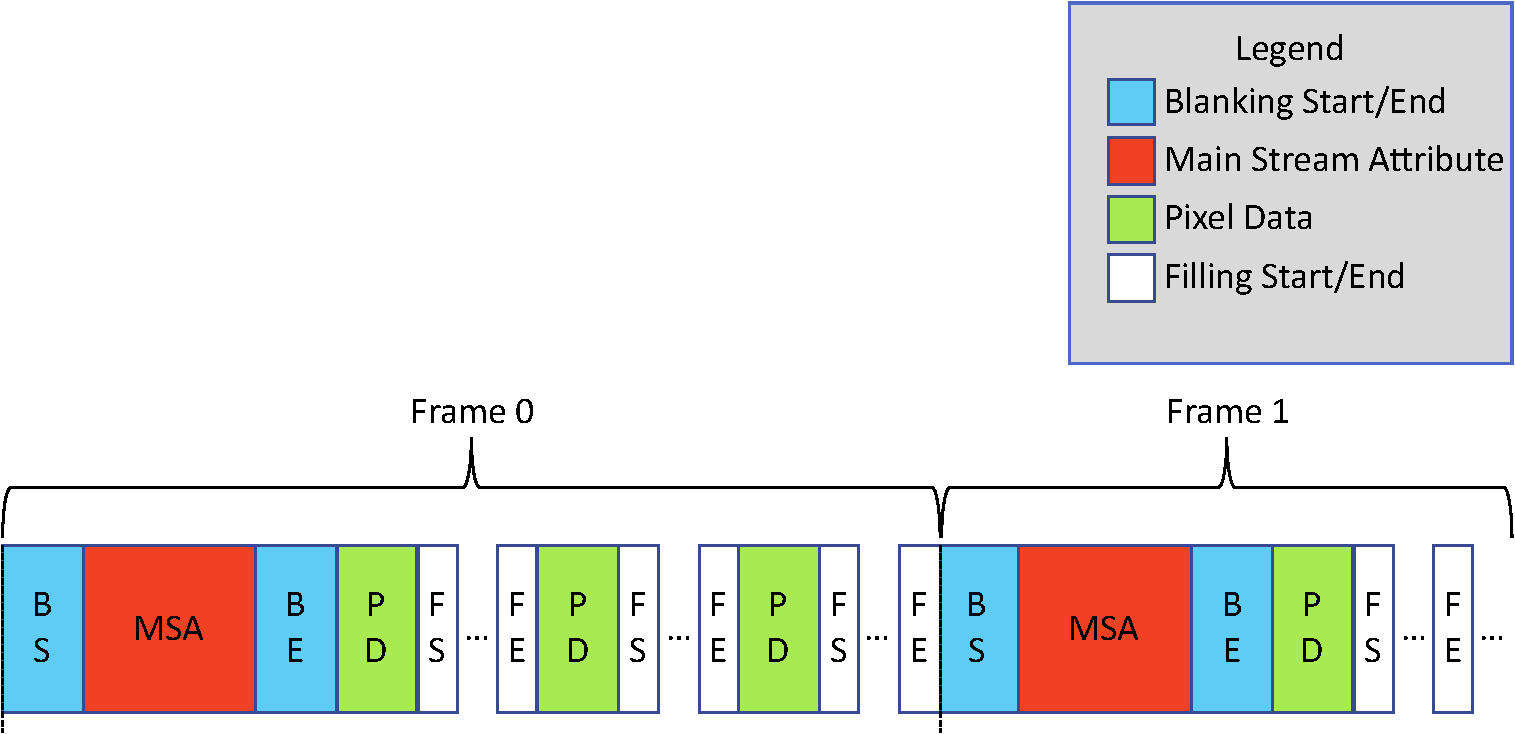
\includegraphics[width=1.0\textwidth]{fig/display_port_framing.pdf}
        \caption{Display Port Framing}
        \label{fig:display_port_framing}
    \end{figure}

    This differs from the PDP in that the PDP allows for completely arbitrary packets to be sent and decoded with differing packet sizes which gives the PDP the ability to support dynamic sub-frame frame rates, and to be extendable to future packet types. Additionally, the PDP carries no internal notion of horizontal or vertical blanking intervals which allows the PDP to operate as fast as possible and give scene generators direct control over frame rates at the user level. For example, the transport upon which the PDP is implemented can operate at the maximum possible data rate allowable in hardware; then, the user in turn can send packets over the data link at the desired rate while inserting empty space where necessary. In the backend, a PDP decoder would decode the data as quickly as possible and display it. From a higher level, this could be viewed as the user issuing commands to send data packets similar to that of how TCP based programs send data over a link with a remote environment executing the actual commands. It is up to the user where and when they want data displayed which enables the PDP to fit a larger set of use cases, and to be simpler to integrate within projector systems.

\section{Packet Format}
    \label{sec:packet_format}
    Given the goals discussed in Chapter~\ref{sec:design_methodology}, it is important to discuss different considerations for packet formatting within the PDP. At a minimum, the PDP needs a method to be able to write to different regions of a display in insolation from other regions. For a region write, a minimal set of data that needs to be encoded is an x start address, y start address, x end address, y end address, and the pixels data. Additionally, these fields need to be able to be efficiently encodable and decodable as well as minimize the necessary intermediate operations required for manipulating the data in both backend architectures (close to an array), and front-end architectures (close to a scene generator). Moreover, the bit-width is important both in terms of encoding/decoding efficiency and rollover. The latter, due to the maximum sizes arrays could reach in terms of resolution.

    Given that majority of off the shelf computer hardware architectures are at least byte aligned or 8-bit aligned in terms of instruction set architecture (ISA) and bus widths, it is prudent to consider data alignment. This is primarily due to unaligned data requiring additional operations such as bit shifting and masking in order to manipulate it within the majority of modern architectures. For example, a multiplication of a 6-bit width data may require storing the result in an 8-bit word and masking the two upper bits to zero before the multiplication operation is performed.

    The coordinate system being utilized within the PDP is another important consideration because sub-optimal choices could lead to unnecessary translations which increase operation costs and computational complexity for manipulating data. For example, if one were to store the beginning X coordinate within a packet with a coordinate offset for the range instead of the end coordinate itself, then computing the ending coordinate for the range would require an addition on the backend. And potentially, $2N^2$ additional mathematical operations to allow comparing region boundaries if the PDP were being composited where N is the number of independent regions to draw.

\section{Packet Types}
    \label{sec:packet_types}
    Table~\ref{tbl:packets} shows the basic packets used for communication within the PDP. These are strictly for data transfer and synchronization of system operations, and do not include other aspects such as system setup or enumeration\footnote{System setup and enumeration are typically system specific operations and outside of the current PDP Design but may be incorporated in the future.}. These packets are organized into type specific fields of some set word-size. The exact size of word fields is left abstracted to allow for an optimal implementation to be used in practice. For example, a system may utilize 24-bit word size if an array has a native 24-bit pixel size, or 32-bit word size if the hardware transport layer has a specific optimal word size. Typically, a multiple of 8-bit word size would be utilized in practice, as most hardware architectures (such as x86) utilize some multiple of this size~\cite{HennessyEtAl2012}. In any given implementation, the word size of all fields must match, in order to simplify decoding operations. This allows for fixed-size decoding of incoming data, which simplifies processing and firmware implementation as well as can ease timing constraints and enforce non-variability in the decoding time of incoming packets of data. In general, PDP packets are designed to send a minimal amount of header data to lower overhead and to allow for pixel orderings that minimize buffering requirements in order to enable real-time processing.

    \begin{table}
        \centering
        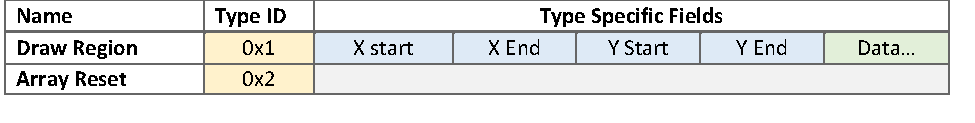
\includegraphics[width=0.9\textwidth]{fig/packet_chart.pdf}
        \caption{List of PDP Packets}
        \label{tbl:packets}
    \end{table}

    In terms of the protocol itself, the PDP uses a single global coordinate system to refer to pixel locations on a display array. For example, a 512 by 512-pixel array would have coordinates from 0 to 511 in both the horizontal and vertical directions. All packets referencing sub-regions of this display would utilize coordinates that map to some rectangular sub-region of the display. Any overlapping regions of data would be composited during system operation with the compositor giving priority to data segments that need to be displayed at higher frame rates.

    PDP Packets are divided into four types, a no operation packet, a draw region packet, array reset packet, and trigger packet. All packets consist of a Type ID field of word-size. The type ID is used by the decoder to determine the packet type.

    The first packet type, {\it No Operation}, is reserved to indicate that command IDs of 0x0 are ignored.

    The second packet type, {\it Draw Region}, is used to send a rectangular sub-region of pixel data in global array coordinates to minimize computations and translations. It has fields for the start and stop horizontal and vertical coordinates (defined inclusively) followed by individual pixel data. For example, suppose a scene generator were to send a packet of data from array region 10 to 19 along the X axis and 20 to 29 along the Y axis, a total of 100 pixels of data would follow the packet coordinates given that the packet specifies a 100 pixel sized region.

    The third packet type, {\it Array Reset}, is utilized to indicate that quadrants on a given array should be cleared. The causes a quadrant to stop displaying its current contents. It consists of an array specific quadrant bitmask used to indicate which quadrant to reset. Any unused bits are reserved. This type of packet would be utilized exclusively to control clearing of quadrants which may be necessary on certain types of array architectures.

    The fourth packet type, {\it Trigger}, could be used to implement a trigger-based synchronization within the PDP. It consists of a system specific action bitmask used to indicate the type of operation to trigger. In IRLED array systems, the coordinator of synchronization is dependent on the array itself and the different components within the system. In some systems, a sensor may be used as the source of synchronization, in other systems, another component may be utilized. Other aspects of system operation may even be triggered outside of the system synchronization interval based off other events. For this reason, the PDP has opted for a trigger-based approach to synchronization. This approach allows for synchronization, data transfer, and computation to be custom tailored for specific use cases. For example, the action mask could be used to trigger the generation of the next frame to be displayed when needed, the source of which is defined by the system itself. Another example would be to utilize the action mask to indicate that further computations (such as scene generation) stall until otherwise indicated.

\section{PDP Stream Decoding}
    \label{sec:pdp_stream_decoding}
    In this section, a discussion of how the PDP might operate with actual data is provided to aid the reader with understanding of how packet decoding is envisioned to work. An actual implementation of the PDP on a real system is discussed in Chapter~\ref{chap:implementation} with experimental results discussed in Chapter~\ref{chap:experimental_results}.

    Figure~\ref{fig:pdp_stream} demonstrates a PDP stream for an architecture with a minimum write size of four pixels and a column-first write order. Data is streaming to the left. Cycles are represented moving downwards with the internal PDP state and pixel buffer data changing as each word is streamed in.

    \begin{figure}
        \centering
        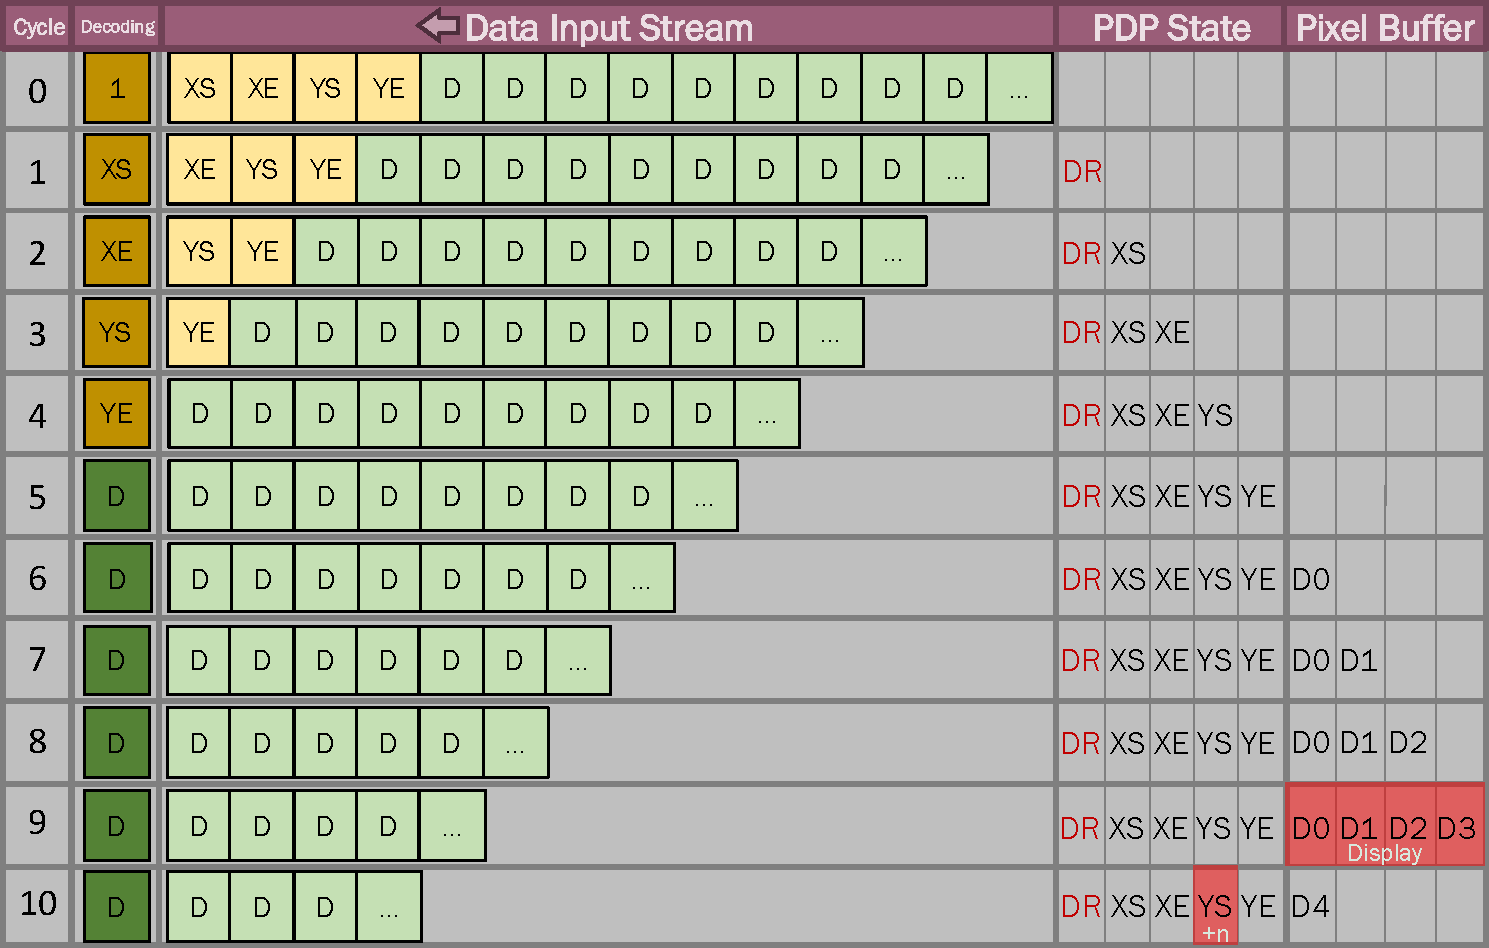
\includegraphics[width=1.0\textwidth]{fig/pdp_stream.pdf}
        \caption{Example PDP Stream}
        \label{fig:pdp_stream}
    \end{figure}

    {\it One} is the command ID for a draw region packet. {\it XS} stands for x start. {\it XE} stands for x end. {\it YS} stands for y start. {\it YE} stands for y end. These are the header words for a PDP draw region packet. {\it D} stands for data which represents each pixel word to draw to an array. At the beginning of time, the PDP state is empty. Once the command ID is decoded, the PDP firmware enters the draw region state indicated by {\it DR}. Then each word for the region boundaries is read in until the entire header has been parsed. Next, pixel data is streamed in starting with {\it D0}. Once all the words necessary for a single array draw are buffered in, the buffered data is then clocked out of the buffer for display. Following this, {\it YS} is incremented to move to the next address on the array\footnote{Array write processes can differ as indicated in Chapter~\ref{sec:array_Interleaved_write_process}, due to this the index {\it n} in Figure~\ref{fig:pdp_stream} is an array specific value that indicates the amount by which to increment {\it YS}. In architectures with a row-first write order, {\it XS} may be incremented instead.}, and {\it D4} is buffered in. Note, an implementation could both display pixels and buffer new pixels for display simultaneously.

    Not shown in the in figure, the buffering and writing process would then continue until the end of the column when {\it YS} equals {\it YE}. Then {\it XS} would be incremented and {\it YS} reset to the start of the region. Then each column would be buffered and written in the same manner as the first until {\it YS} equals {\it YE} and {\it XS} equals {\it XE}, which indicates the end of the frame. After this, a new packet would be streamed in and decoded in the same manner.

    One important note about the decoding process discussed here is that it would be relatively simple to implement by utilizing a state machine within hardware that encapsulates the different PDP state variables. A major factor in this is the fixed width word size utilized within the PDP. Fixed width decoding means that partial words do not need to be buffered, and dynamic buffers and routing need not be utilized within a decoder. As discussed in Chapter~\ref{sec:design_methodology}, one of the design goals of the PDP is to provide a means to ease implementation complexity. This simplification of hardware implementation allows for resources to be focused on optimally routing data in and out of the an FPGA, ASIC, or other implementations while minimizing timing closure issues in an environment where a major challenge is the plethora of signals that need to be routed. For example, within NSLEDS and HDILED based systems, it is necessary to route 512 data lines due to the 32 16-bit DAC channels used. Future systems could double that number to 1024 by utilizing 64 16-bit DAC channels.

    As one of the goals of the PDP is to provide backwards compatibility, an important consideration is how this decoding process might be implemented within a display protocol transport layer. Most of the details regarding this is discussed in Chapter~\ref{sec:hdmi_transport_layer}. For now, it is worth noting that for an implementation that is backwards compatible with HDMI, draw packet headers could be transmitted by a secondary data channel while leaving the main stream channel for pixel data. This would allow for pixels data to be transmitted exactly as normal while utilizing normal display protocol modelines, thus, allowing users to be able to utilize their array technology transparently as-is without any changes while utilizing an array that internally supports the PDP via its close support electronics.

\section{Overhead}
    As mentioned previously, internally the PDP has no notion of blanking periods or porches for providing synchronization, and therefore does not encapsulate the inefficiencies inherent in the aforementioned protocols. Instead synchronization and frame rates within the PDP are controlled by the source through timing when data is sent. This means that high overheads due to blanking can be mitigated. Table~\ref{tbl:pdp_efficiency} shows the maximum packet overhead due to packet encapsulation when the PDP is utilized for the same resolutions and frequencies listed in Table~\ref{tbl:modeline_overhead}. These are computed using active pixel area over total pixel area. The original modeline overheads are shown in the {\it Modeline Overhead} column. The {\it Overhead Reduction} columns show the percent reduction relative to the original modeline for both bit-packed and unpacked data. Note, unpacked data requires buffering double the number of pixels in order to write the same amount of data to an array as bit-packed data so one would need to double the modeline size in practice.

    \begin{table}
        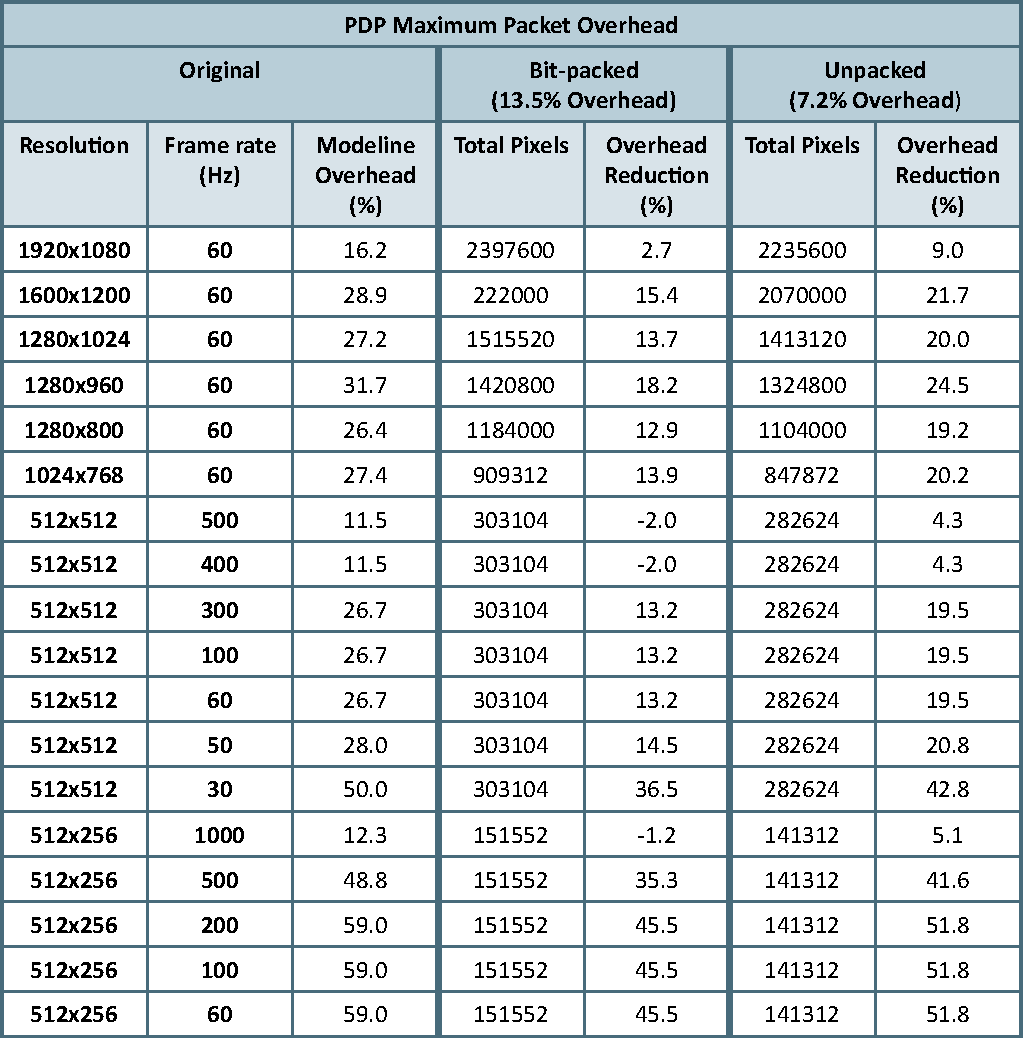
\includegraphics[width=1.0\textwidth]{fig/maximum_packet_overhead.pdf}
        \caption{PDP Maximum Packet Overhead}
        \label{tbl:pdp_efficiency}
    \end{table}

    {\it 512 by 512} and {\it 512 by 256} are typical modeline resolutions used on IRLED arrays. These numbers represent a worst-case scenario when the PDP is implemented within a transport layer that does not require blanking intervals. In actual usage, larger packets consisting of more pixels would be utilized therefore, the overhead would be lower on average. However, even in worst-case scenarios the PDP has a vast reduction on bandwidth requirements on average which means that faster refresh rates can be utilized in bandwidth limited situations. Additionally, higher integration times could be utilized within IR cameras and sensors due to less time being needed for writing the same visible data to an IR array. For example, with the 512 by 256 modeline operating at \mbox{200 hertz}, integration time could be increased by up to 45.5 percent over a traditional modelines for bit-packed data.

    The numbers in Table~\ref{tbl:pdp_efficiency} are computed by taking the visible resolution and dividing it by the minimum pixel write size supported on an array. The minimum pixel write size is also synonymous with the minimum possible PDP packet payload size excluding headers, and thus, is denoted as $S_{pkt}$. This yields the maximum possible packet count, $C_{pkt}$, for a given resolution as shown in Equation~\eqref{eq:packet_max}. The visible resolution parameters are denoted as horizontal active, $h_a$, and vertical active, $v_a$, respectively to keep consistent with the naming conventions used in Chapter~\ref{chap:display_protocols}. Within the NSLEDS and HDILED arrays, the minimal packet size for packed data, $S_{pktP}$, is 2 by 16 due to the interleaved array write process and bit-packing format discussed in Chapter~\ref{chap:array_write_process}. The minimal packet size for unpacked data, $S_{pktU}$, is 2 by 32 pixels due to unpacked data needing double the amount of pixel data per write.

    \begin{equation}
        \begin{array}{ l }
            \displaystyle C_{pkt}=\frac{h_a \cdot v_a}{S_{pkt}} \\[13pt]
            \displaystyle C_{pkt_P}=\frac{h_a \cdot v_a}{2 \cdot 16}\\[13pt]
            \displaystyle C_{pkt_U}=\frac{h_a \cdot v_a}{2 \cdot 32}\\[13pt]
        \end{array}
        \label{eq:packet_max}
    \end{equation}

    The total pixel overhead, $O_{px}$, is computed by multiplying the total packet count, $C_{pkt}$, by the packet overhead, $O_{pkt}$, as shown in Equation~\eqref{eq:overhead_pixel}. The overhead is determined by looking at the total number of additional words added for PDP header data. Header details are discussed in Chapter~\ref{sec:packet_format}.

    \begin{equation}
        \begin{array}{ l }
            \displaystyle O_{px}=O_{pkt} \cdot C_{pkt} \\
            \displaystyle O_{px}=5\cdot C_{pkt} \\[13pt]
        \end{array}
        \label{eq:overhead_pixel}
    \end{equation}

    The total pixel count, $T_{px}$, is determined by adding the total pixel overhead, $O_{px}$, (or the result of Equation~\eqref{eq:overhead_pixel}) to the visible pixel size as shown in Equation~\eqref{eq:total_pixel}.

    \begin{equation}
        \begin{array}{ l }
            \displaystyle T_{px}=O_{pkt} \cdot C_{pkt} + h_a \cdot v_a \\
            \displaystyle T_{px}=O_{px} + h_a \cdot v_a \\
            \displaystyle T_{px}=5\cdot C_{pkt} + h_a \cdot v_a \\[13pt]
        \end{array}
        \label{eq:total_pixel}
    \end{equation}

    Putting the input variables together and simplifying yields Equation~\eqref{eq:total_pixel2} where $T_{px}$ is the total pixel count.

    \begin{equation}
        \begin{array}{ l }
            \displaystyle T_{px}=O_{pkt} \cdot \frac{h_a \cdot v_a}{S_{pkt}} + h_a \cdot v_a \\[13pt]
            \displaystyle T_{px}=h_a \cdot v_a \cdot (\frac{O_{pkt}}{S_{pkt}} + 1) \\[13pt]
            \displaystyle T_{px_P}=h_a \cdot v_a \cdot (\frac{5}{2 \cdot 16} + 1) \\[13pt]
            \displaystyle T_{px_U}=h_a \cdot v_a \cdot (\frac{5}{2 \cdot 32} + 1) \\[13pt]
        \end{array}
        \label{eq:total_pixel2}
    \end{equation}

    Equation~\ref{eq:overhead} shows computing the overhead percentage, $O_{pdp}$, is a matter of dividing the total pixel overhead, $O_{px}$, by the total pixels, $T_{px}$.

    \begin{equation}
        \begin{array}{ l }
            \displaystyle O_{pdp}=\frac{O_{pkt}\cdot C_{pkt}}{T_{px}} \cdot 100 \\[13pt]
            \displaystyle O_{pdp}=\frac{O_{px}}{T_{px}} \cdot 100 \\[13pt]
        \end{array}
        \label{eq:overhead}
    \end{equation}

    Due to the nature of the total pixel overhead being proportional to the visible pixel size for each resolution, the overhead percentage under worst-case conditions cancels out to a constant consisting of only a relationship between the minimum packet size and packet overhead. Substituting Equations~\ref{eq:packet_max} and~\ref{eq:total_pixel2} into Equation~\ref{eq:overhead} yields Equation~\ref{eq:cancel} which shows this cancellation process and the resulting overhead percentages. The overhead for packed data is $13.5\%$ and the overhead for unpacked data is $7.2\%$.

    \begin{equation}
        \begin{array}{ l }
            \displaystyle O_{pdp}=\frac{O_{pkt}\cdot \frac{h_a \cdot v_a}{S_{pkt}}}{O_{pkt} \cdot \frac{h_a \cdot v_a}{S_{pkt}} + h_a \cdot v_a} \cdot 100 \\[16pt]
            \displaystyle O_{pdp}=\frac{O_{pkt}\cdot \frac{\cancelto{1}{h_a \cdot v_a}}{S_{pkt}}}{O_{pkt} \cdot \frac{\cancelto{1}{h_a \cdot v_a}}{S_{pkt}} + \cancelto{1}{h_a \cdot v_a}} \cdot 100 \\[25pt]
            \displaystyle O_{pdp}=\frac{O_{pkt}\cdot \frac{1}{S_{pkt}}}{O_{pkt} \cdot \frac{1}{S_{pkt}} + 1} \cdot 100 \\[16pt]
            \displaystyle O_{pdp}=\frac{\frac{O_{pkt}}{S_{pkt}}}{\frac{O_{pkt}}{S_{pkt}} + 1} \cdot 100 \\[19pt]
            \displaystyle O_{pdp}=\frac{O_{pkt}}{O_{pkt}+S_{pkt}} \cdot 100 \\[19pt]
            \displaystyle O_{pdp_P}=\frac{5}{5 + 2 \cdot 16} \cdot 100 \\[19pt]
            \displaystyle O_{pdp_P}=13.5 \\[13pt]
            \displaystyle O_{pdp_U}=\frac{5}{5 + 2 \cdot 32} \cdot 100 \\[19pt]
            \displaystyle O_{pdp_U}=7.2 \\[13pt]
        \end{array}
        \label{eq:cancel}
    \end{equation}

    The overhead reduction in Table~\ref{tbl:pdp_efficiency} is computed by subtracting the PDP overhead from the overheads listed in Table~\ref{tbl:modeline_overhead}. In most cases, there is an overhead reduction. It is worth restating for posterity that these numbers represent worst-case scenarios for the PDP when implemented on top of a transport layer that does not require blanking intervals. If the underlying transport layer upon which the PDP is implemented cannot function without additional overhead, then the performance would be worse in practice as is the case if the PDP is utilized with a display protocol-based transport layer. However, in the case of display protocols, overhead can be minimized relative to normal non-PDP operation by utilizing the fastest frequency the hardware allows and minimizing modeline porches. This would enable the PDP to use much smaller porches than normal modelines. Additionally, horizontal porch overhead can be mitigated by timing any inherit analog settling delays to occur during porches. This can be done by ensuring that there is enough data for a write prior to a horizontal blanking period.

\section{Multi-frame Rate Performance}
    \label{sec:multi_framerate_performance}

    This section discusses the benefits of utilizing a PDP based approach for reaching high frame rates. In high performance systems, data movement~\cite{LeeEtAl1984}, bandwidth~\cite{LaiBaker1999}, and latency~\cite{ZhengEtAl2014} are of primary concern due to the nature of these typically impeding performance requirements. In many cases, minimizing data movement can vastly improve the performance of systems~\cite{BandyopadhyayCoyle2004,LiEtAl2009,Hall2020}. In real time systems~\cite{Kopetz2011}, such as IR projector systems, where end-to-end latency is important for driving arrays, and the observation of real-time IR behavior is important for characterizing temperature changes~\cite{ZhouEtAl2000} minimizing data movement, and choosing appropriate hardware with high bandwidth as well as low-latency is extremely important.

    As detailed throughout this dissertation, the PDP allows for control over which individual segments of an array can be written to. This means that large amounts of bandwidth can be saved by updating parts of a frame at slower frame rates than other sections of a frame. In a simplified dual frame rate setup, Equation~\eqref{eq:bandwidth_saved} and the subsequent simplification show how to compute the percentage of saved bandwidth, $b_s$, when operating some proportion of pixels at a slower rate than a given faster rate. The proportion of pixels operating at a slow frame rate is $p$, the fast frame rate is $r_f$, and the slow frame rate is $r_s$. The final simplified form is the percentage of pixels operating at a slow rate multiplied by the difference between the rates over the fast rate.

    \begin{equation}
        \begin{array}{ l }
            \displaystyle b_s=\left(1-\frac{(1-p)\cdot r_f + p\cdot r_s}{r_f}\right)\cdot 100 \\[16pt]
            \displaystyle b_s \cdot r_f=\left(r_f-r_f \cdot \frac{(1-p)\cdot r_f + p\cdot r_s}{r_f}\right)\cdot 100 \\[13pt]
            \displaystyle b_s \cdot r_f= (r_f - (1-p)\cdot r_f - p\cdot r_s)\cdot 100 \\[13pt]
            \displaystyle b_s \cdot r_f= (r_f - r_f + p \cdot r_f - p\cdot r_s)\cdot 100 \\[13pt]
            \displaystyle b_s \cdot r_f= (p \cdot r_f - p\cdot r_s)\cdot 100 \\[13pt]
            \displaystyle b_s \cdot r_f= (p \cdot (r_f - r_s))\cdot 100 \\[13pt]
            \displaystyle b_s=\left(\frac{p \cdot (r_f-r_s)}{r_f}\right)\cdot 100
        \end{array}
        \label{eq:bandwidth_saved}
    \end{equation}

    Table~\ref{tbl:multi_framerate_bandwidth_savings} shows various examples of the bandwidth saved relative to operating all pixels at a given fast frame rate for PDP operation when two frame rates are utilized. The results are computed using Equation~\eqref{eq:bandwidth_saved} to give the reader an understanding of the kinds of savings that are possible by utilizing this method of operation. Of note, driving just half of the pixels at a slow rate can save near 50 percent of the bandwidth in these scenarios. This is of particular importance because many types of IR test scenarios utilized in practice contain sparse objects with low intensity backgrounds. In these types of scenarios, the bandwidth reduction would translate into the ability to display fast imagery at much higher rates than possible with conventual display technology. Indeed, display of small objects could have bandwidth reductions of over 95 percent. While these equations demonstrate a simplified use case for the PDP, they provide a powerful argument for why the intra-frame variable refresh rate technology within the PDP has the potential to provide orders of magnitude better performance in bandwidth starved environments. In practice, many current projector systems struggle to achieve frame Rates above \mbox{200 hertz} due to the inability to deliver data at higher rates when utilizing conventional display technology.

    \begin{table}
        \centering
        \large
        \begin{tcolorbox}[tabularx={Y|Y|Y|Y},title=\textbf{Multi-frame Rate Bandwidth Savings},boxrule=0.5pt]
        \textbf{\normalsize Slow Frame Rate (Hz)} & \textbf{\normalsize Fast Frame Rate (Hz)} & \textbf{\normalsize Proportion of Slow Pixels (p)} & \textbf{\normalsize Bandwidth Saved (\%)} \\ \hline
            \textbf{\normalsize 10} & \textbf{\normalsize 100} & {\normalsize 0.1} & {\normalsize 9.0} \\ \hline
            \textbf{\normalsize 10} & \textbf{\normalsize 100} & {\normalsize 0.2} & {\normalsize 18.0} \\ \hline
            \textbf{\normalsize 10} & \textbf{\normalsize 100} & {\normalsize 0.3} & {\normalsize 27.0} \\ \hline
            \textbf{\normalsize 10} & \textbf{\normalsize 100} & {\normalsize 0.4} & {\normalsize 36.0} \\ \hline
            \textbf{\normalsize 10} & \textbf{\normalsize 100} & {\normalsize 0.5} & {\normalsize 45.0} \\ \hline
            \textbf{\normalsize 10} & \textbf{\normalsize 100} & {\normalsize 0.6} & {\normalsize 54.0} \\ \hline
            \textbf{\normalsize 10} & \textbf{\normalsize 100} & {\normalsize 0.7} & {\normalsize 63.0} \\ \hline
            \textbf{\normalsize 10} & \textbf{\normalsize 100} & {\normalsize 0.8} & {\normalsize 72.0} \\ \hline
            \textbf{\normalsize 10} & \textbf{\normalsize 100} & {\normalsize 0.9} & {\normalsize 81.0} \\ \hline
            \textbf{\normalsize 10} & \textbf{\normalsize 100} & {\normalsize 1.0} & {\normalsize 90.0} \\ \hline
            \textbf{\normalsize 10} & \textbf{\normalsize 1000} & {\normalsize 0.1} & {\normalsize 9.9} \\ \hline
            \textbf{\normalsize 10} & \textbf{\normalsize 1000} & {\normalsize 0.2} & {\normalsize 19.8} \\ \hline
            \textbf{\normalsize 10} & \textbf{\normalsize 1000} & {\normalsize 0.3} & {\normalsize 29.7} \\ \hline
            \textbf{\normalsize 10} & \textbf{\normalsize 1000} & {\normalsize 0.4} & {\normalsize 39.6} \\ \hline
            \textbf{\normalsize 10} & \textbf{\normalsize 1000} & {\normalsize 0.5} & {\normalsize 49.5} \\ \hline
            \textbf{\normalsize 10} & \textbf{\normalsize 1000} & {\normalsize 0.6} & {\normalsize 59.4} \\ \hline
            \textbf{\normalsize 10} & \textbf{\normalsize 1000} & {\normalsize 0.7} & {\normalsize 69.3} \\ \hline
            \textbf{\normalsize 10} & \textbf{\normalsize 1000} & {\normalsize 0.8} & {\normalsize 79.2} \\ \hline
            \textbf{\normalsize 10} & \textbf{\normalsize 1000} & {\normalsize 0.9} & {\normalsize 89.1} \\ \hline
            \textbf{\normalsize 10} & \textbf{\normalsize 1000} & {\normalsize 1.0} & {\normalsize 99.9} \\ \hline
        \end{tcolorbox}
        \caption{Multi-frame Rate Bandwidth Savings}
        \label{tbl:multi_framerate_bandwidth_savings}
    \end{table}

    Now that the PDP design methodology, underlying protocol details, performance characteristics, and potential operation within a system have been explored. Discussion is shifted to the machine model upon which the PDP operates to show the generalized type of environment the PDP is envisioned to be utilized within in the future.
